\documentclass[a4paper,12pt]{article}
\usepackage{graphicx}
\usepackage{titling}
\usepackage[margin=1in]{geometry}
\usepackage{setspace}
\usepackage{amsmath}
\setstretch{1.5}
\graphicspath{{images/}}
\begin{document}

% Cover page content
\begin{titlepage}
    \centering

    {\scshape\LARGE Posts and Telecommunications Institute of Technology \par}
    \vspace{2cm}
    
    {\scshape\Large Course Title: Python \par}
    \vspace{1.5cm}
    
    {\huge\bfseries Project Title: Python Programming\par}
    \vspace{2cm}
    
    {\Large\bfseries Student Name: Cao Ngoc Huy\par}
    \vspace{0.5cm}
    {\Large\bfseries Student ID: B23DCCE043\par}
    \vspace{0.5cm}
    
    {\Large\bfseries Instructor Name: Kim Ngoc Bach\par}
    \vfill
    
    {\Large Date of Submission: 03/05/2025\par}
\end{titlepage}
\newpage

\section*{List of Sections}
\begin{enumerate}
    \item\textbf{Introduction}
    \item \textbf{Collecting football player statistical data of English Premier League}
    
    \item \textbf{Data Analysis}
    \begin{enumerate}
        \item Identify the top 3 players with the highest and lowest for each statistic
        \item Find the median, calculate the mean and standard deviation
        \item Plot histogram showing the distribution of each statistic for all players
        \item Identify the highest score team
    \end{enumerate}
    
    \item \textbf{Clustering}
    \begin{enumerate}
        \item Plot 2D cluster of the data points
    \end{enumerate}
    
    \item \textbf{Player Value Estimation}
    \begin{enumerate}
        \item Collect player transfer values for the 2024-2025 season
        \item Propose a method for estimating player value
    \end{enumerate}
    \item\textbf{Conclusion}
\end{enumerate}

\newpage

\section{Introduction}

In recent years, data analytics has played an increasingly important role in professional sports, particularly in football (soccer). Statistical data is now widely used by clubs, analysts, and fans to assess player performance, optimize team strategies, and guide financial decisions such as player transfers. This project focuses on using Python programming to collect, process, and analyze football player statistics from the 2024–2025 English Premier League season.

The primary goal of the project is to develop a system that collects a wide range of player performance metrics from publicly available data sources. These metrics include general playing time, goals, assists, expected goals (xG), defensive actions, passing statistics, and more. Players with more than 90 minutes of playing time are included in the dataset, which is retrieved from \texttt{fbref.com}, a well-known football statistics site. The dataset is saved in a structured format as \texttt{results.csv}.

The second goal is to analyze the data statistically. This includes identifying the top performers, calculating statistical summaries such as mean, median, and standard deviation, and visualizing the data distribution using histograms. Additionally, the project aims to determine which team performs best based on aggregated statistics.

Furthermore, clustering techniques are applied using the K-Means algorithm, combined with Principal Component Analysis (PCA), to group players based on their performance attributes and visualize these clusters in a 2D plot.

Finally, the project collects player transfer values from \texttt{footballtransfers.com} and proposes a machine learning approach (using Random Forest Regression) to estimate player market values based on their in-game statistics. This includes preprocessing, feature selection, model training, and evaluation using metrics such as mean squared error (MSE).

This project not only provides practical experience in data science using Python, but also illustrates how statistical and machine learning methods can be applied to real-world sports analytics.

\newpage

\section{Collecting football player statistical data of English Premier League}

The data is collected from the following web pages of the FBRef website:
\begin{itemize}
    \item \texttt{stats\_standard}: General player statistics
    \item \texttt{stats\_keeper}: Goalkeeper statistics
    \item \texttt{stats\_shooting}: Shooting statistics
    \item \texttt{stats\_passing}: Passing statistics
    \item \texttt{stats\_gca}: Goal Creation Actions (GCA) statistics
    \item \texttt{stats\_defense}: Defensive statistics
    \item \texttt{stats\_possession}: Possession statistics
    \item \texttt{stats\_misc}: Miscellaneous statistics
\end{itemize}

The URLs for these pages are stored in a dictionary for easy access.

\subsection{Data Preprocessing}

\subsection{Web Scraping}

The web scraping is performed using the Python libraries \texttt{requests} and \texttt{BeautifulSoup}. The process follows these steps:

\begin{enumerate}
    \item Send an HTTP request to the target URL using the \texttt{requests} library.
    \item Parse the returned HTML content using \texttt{BeautifulSoup}.
    \item Remove unnecessary comments in the HTML to clean up the data.
    \item Find the relevant table in the HTML structure using the \texttt{find()} function.
\end{enumerate}

\subsection{Extracting Table Headers}

The table headers are extracted from the \texttt{thead} section of the table. Each header corresponds to a specific statistical category for players, such as \texttt{player}, \texttt{nationality}, \texttt{team}, etc. The headers are filtered to only include the relevant statistics defined in the \texttt{target} list.

\subsection{Extracting Data Rows}

The rows of data are extracted from the \texttt{tbody} section. Each row contains the statistics for a player. The values are mapped to their corresponding headers. Special handling is applied to the \texttt{minutes} field, converting it into an integer. Missing values are handled by inserting "N/a".

\subsection{Data Merging}

After scraping the data from the different stat groups, the individual DataFrames are merged into a single DataFrame.

\subsection{Merge Keys}

The key columns used for merging the data are \texttt{player} and \texttt{team}. The merging is performed sequentially across the stat groups using the \texttt{merge()} function in pandas.

\subsection{Merging Process}

For each stat group (except for the \texttt{stats\_standard} group, which serves as the base), the relevant columns are selected. The columns that already exist in the merged DataFrame are dropped, while the columns that are not present are added. The data is merged using a left join, ensuring that all player information is retained.

\subsection{Cleaning the Data}

After merging, the following cleaning steps are performed:
\begin{itemize}
    \item Missing values are filled with "N/a".
    \item Players who have played less than 90 minutes are filtered out.
    \item The columns are reordered according to the \texttt{target} list.
\end{itemize}

\subsection{Final Output}

The final cleaned and merged DataFrame is sorted by \texttt{player} name and the column names are renamed using a predefined dictionary (\texttt{target\_name\_dict}). The final dataset is saved to a CSV file titled \texttt{results.csv}.


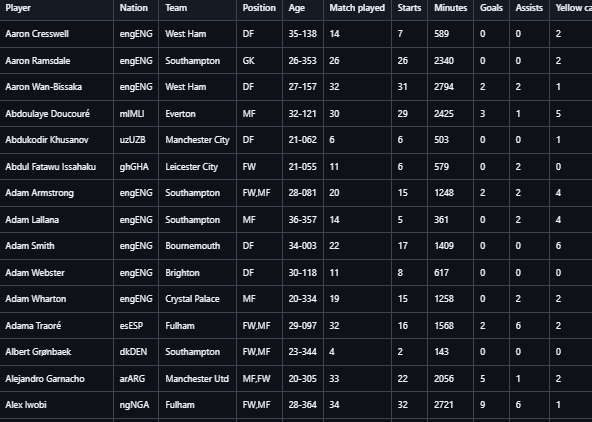
\includegraphics{results.png}



\newpage

\section{Data analysis}

\subsection{Identify the Top 3 Players with the Highest and Lowest for Each Statistic}

This section outlines the methodology used to identify the top 3 players with the highest and lowest values for each statistic in the dataset. The goal is to provide insights into the best and worst performers for each statistical category.

\subsubsection{Loading the Data}

The first step is to load the merged dataset from the CSV file generated in the previous step. This dataset contains various statistics for each player, which are stored in a structured format with columns representing different statistical categories.

\begin{verbatim}
merged_df = pd.read_csv('results.csv')
\end{verbatim}

The dataset is loaded into a pandas DataFrame, and we begin the analysis by replacing any instances of "N/a" with zeros. This is done to ensure that missing values do not interfere with the analysis.

\begin{verbatim}
merged_df = merged_df.replace('N/a', 0)
\end{verbatim}

\subsubsection{Age Conversion to Days}

Next, the \texttt{Age} column is processed. Age values, represented in the format "XX years YY days", are converted into the total number of days for easier comparison. The conversion formula is:

\[
\text{Total Age in Days} = (XX \times 365) + YY
\]

This step allows us to work with a single unit of measurement (days) for age comparisons. The code snippet below handles this conversion:

\begin{verbatim}
for i in merged_df['Age']:
    cell = str(i)
    temp = int(cell[0:2])* 365 + int(cell[3:])
    i = temp
\end{verbatim}

This loop processes each player's age, extracts the years and days, and calculates the total age in days.

\subsubsection{Converting Columns to Numeric}

To ensure that statistical operations can be performed, all relevant columns are converted to numeric data types. Any non-numeric values (such as strings or missing data) are coerced into `NaN`, which are then replaced with zeros.

\begin{verbatim}
for col in merged_df.columns[4:]:
    merged_df[col] = pd.to_numeric(merged_df[col], errors='coerce').fillna(0)
\end{verbatim}

This conversion is applied to the statistics columns (starting from index 4) to ensure that calculations like sorting and comparisons are valid.

\subsubsection{Identifying Top and Bottom Performers}

The core of this methodology is to identify the top 3 players with the highest and lowest values for each statistic. This is achieved by iterating through each statistical column and using pandas' built-in functions to retrieve the top 3 largest and smallest values for each column.

For each statistic, the following steps are performed:

1. **Skip empty statistics**: If a statistic has no meaningful data (i.e., all values are zero), it is skipped.
2. **Find the top 3 players**: Using \texttt{nlargest()} to find the top 3 highest values and \texttt{nsmallest()} to find the top 3 lowest values for each statistic.
3. **Format the results**: For each statistic, a list of the top 3 highest and lowest players is created, formatted as a string.

\begin{verbatim}
top_highest = merged_df[['Player', stat]].nlargest(3, stat)
top_lowest = merged_df[['Player', stat]].nsmallest(3, stat)

highest_entries = [f"{row['Player']}: {row[stat]}" for _, row in top_highest.iterrows()]
lowest_entries = [f"{row['Player']}: {row[stat]}" for _, row in top_lowest.iterrows()]

results.append(
    f"Statistic: {stat}\n"
    f"Highest:\n" + "\n".join(highest_entries) + "\n"
    f"Lowest:\n" + "\n".join(lowest_entries) + "\n"
)
\end{verbatim}

\subsubsection{Outputting the Results}

After identifying the top and lowest players for each statistic, the results are stored in a text file named \texttt{top\_3.txt}. The results are formatted into a human-readable format that includes the statistic name, followed by the top 3 highest and lowest players for that statistic.

The results are written into a text file as follows:

\begin{verbatim}
with open('top_3.txt', 'w', encoding = 'utf-8') as f:
    f.write(str_temp)
\end{verbatim}

The final output includes the players' names and their corresponding values for the highest and lowest statistics, organized by statistic.

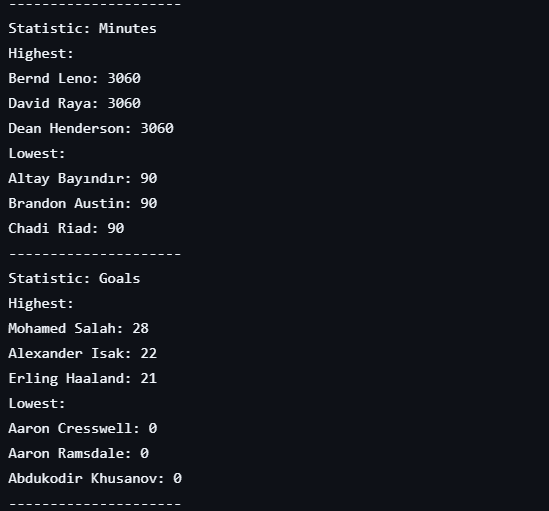
\includegraphics{top3.png}

\subsubsection{Conclusion}

The methodology efficiently identifies the top 3 players with the highest and lowest values for each statistic. This is achieved through:
\begin{itemize}
    \item Data cleaning and conversion, ensuring that the data is in a format suitable for analysis.
    \item Iterating over each statistic to find the top 3 highest and lowest players.
    \item Outputting the results in a clear, readable format for further analysis or reporting.
\end{itemize}

This process provides valuable insights into the players' performances in each statistical category and allows for easy identification of standout performers as well as areas for improvement.






\subsection{Find the median, calculate the mean and standard deviation}
This section outlines the methodology used to calculate the median, mean, and standard deviation for the statistical performance of football players. The goal is to provide an understanding of the distribution of various statistics and how individual teams and players compare to the overall league performance.

\subsubsection{Loading the Data}

The analysis starts by loading the merged dataset, which contains the statistical performance of football players. This dataset, stored in a CSV file named \texttt{results.csv}, is read into a pandas DataFrame.

\begin{verbatim}
merged_df = pd.read_csv('results.csv')
\end{verbatim}

The dataset is then processed by converting the relevant columns to numerical values, where necessary, and replacing any missing data, represented as "N/a", with zeros.

\begin{verbatim}
merged_df[stat_columns] = merged_df[stat_columns].replace('N/a', 0)
\end{verbatim}

Additionally, the \texttt{Age} column is converted to a number representing the total number of days, allowing for easier comparison and analysis.

\begin{verbatim}
age_row = []
for i in merged_df['Age']:
    cell = str(i)
    temp = int(cell[0:2])* 365 + int(cell[3:])
    age_row.append(temp)
merged_df['Age'] = age_row
\end{verbatim}

\subsubsection{Converting Statistical Columns to Numeric}

The next step involves ensuring that all statistical columns are in a numeric format. This is essential for performing mathematical operations such as mean and standard deviation calculations. The non-statistical columns, such as player names and team information, are excluded from this conversion.

\begin{verbatim}
for col in stat_columns:
    merged_df[col] = pd.to_numeric(merged_df[col], errors='coerce').fillna(0)
\end{verbatim}

This conversion ensures that all the statistical data is ready for mathematical analysis.

\subsubsection{Calculating the Median, Mean, and Standard Deviation}

The central part of this methodology is the calculation of three key statistical measures for each of the statistics:

\begin{itemize}
    \item **Median**: The median value for each statistic is calculated using the \texttt{median()} function. The median is a robust measure of central tendency, especially in the presence of outliers.
    \item **Mean**: The mean, or average, is calculated using the \texttt{mean()} function. This measure provides a general sense of the average performance across all players.
    \item **Standard Deviation (Std)**: The standard deviation, calculated using the \texttt{std()} function, measures the variation or dispersion of the statistics. A higher standard deviation indicates greater variability in performance.
\end{itemize}

These calculations are performed for all players in the league and for each team separately. First, the overall league statistics are computed:

\begin{verbatim}
medians = merged_df[stat_columns].median()
means = merged_df[stat_columns].mean()
stds = merged_df[stat_columns].std()
\end{verbatim}

These values are then stored in a dictionary for the league-wide statistics:

\begin{verbatim}
all_stats = {}
for col in stat_columns:
    all_stats[f'Median of {col}'] = medians[col]
    all_stats[f'Mean of {col}'] = means[col]
    all_stats[f'Std of {col}'] = stds[col]
rows.append(all_stats)
\end{verbatim}

\subsubsection{Calculating Statistics for Each Team}

Next, the statistics are calculated for each individual team. The DataFrame is filtered by team, and the same statistical measures are calculated for the players of each team:

\begin{verbatim}
teams = merged_df['Team'].unique()
for team in teams:
    team_df = merged_df[merged_df['Team'] == team]
    team_medians = team_df[stat_columns].median()
    team_means = team_df[stat_columns].mean()
    team_stds = team_df[stat_columns].std()

    team_stats = {}
    for col in stat_columns:
        team_stats[f'Median of {col}'] = team_medians[col]
        team_stats[f'Mean of {col}'] = team_means[col]
        team_stats[f'Std of {col}'] = team_stds[col]
    rows.append(team_stats)
    index_names.append(team)
\end{verbatim}

This allows for a comparison between teams and the league-wide performance. The results for both the league and individual teams are stored in a list.

\subsubsection{Creating the Final DataFrame}

Once the statistical calculations are complete, the results are stored in a pandas DataFrame. The index names for the DataFrame include "all" for the league-wide statistics and the names of each team. This DataFrame is then saved to a CSV file for future reference.

\begin{verbatim}
results_df = pd.DataFrame(rows, index=index_names)
results_df.to_csv('results2.csv', index=index_names)
\end{verbatim}

The resulting CSV file contains the median, mean, and standard deviation for each statistic, both for the entire league and for each individual team.

\subsubsection{Result}
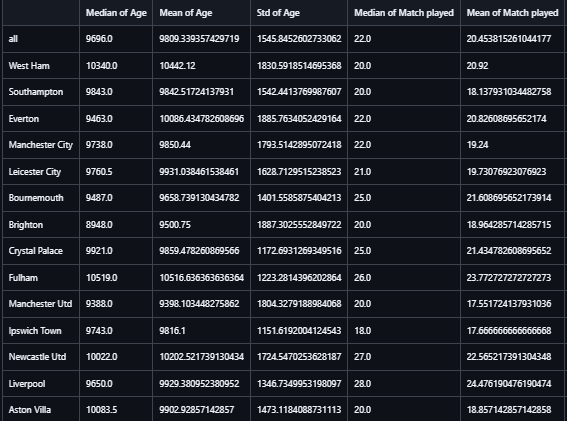
\includegraphics{results2.png}
\subsubsection{Conclusion}

The methodology used in this section enables the calculation of fundamental statistical measures—median, mean, and standard deviation—across different performance metrics. These measures provide a clear overview of the overall performance of players and teams in the league. By calculating these statistics, we can better understand the distribution and variability of player performances and compare them both within teams and across the entire league.


\subsection{Plot histogram showing the distribution of each statistic for all players}
This section describes the methodology used to generate histograms visualizing the distribution of various statistics for football players. The purpose of plotting these histograms is to provide an intuitive understanding of the distribution of performance metrics across all players and individual teams.

\subsubsection{Loading and Preparing the Data}

The analysis begins by loading the dataset from a CSV file named \texttt{results.csv}, which contains the statistical performance of football players. The relevant columns for the statistical measures are selected by excluding the non-statistical columns, such as player names, teams, and positions.

\begin{verbatim}
merged_df = pd.read_csv('results.csv')
non_stat_columns = ['Player', 'Nation', 'Team', 'Position']
stat_columns = [col for col in merged_df.columns if col not in non_stat_columns]
\end{verbatim}

The \texttt{Age} column is converted to a numerical value representing the player's age in years. This step ensures that the data is in a consistent format for analysis.

\begin{verbatim}
age_row = []
for i in merged_df['Age']:
    cell = str(i)
    temp = float(cell[0:2]) + float(int(cell[3:])/365)
    age_row.append(temp)
merged_df['Age'] = age_row
\end{verbatim}

In addition, all the statistical columns are converted to numeric values. Any invalid or missing values are coerced into zero, ensuring that all data can be used in the histogram plotting.

\begin{verbatim}
for col in stat_columns:
    merged_df[col] = pd.to_numeric(merged_df[col], errors='coerce').fillna(0)
\end{verbatim}

\subsubsection{Setting Up Directories for Saving Histograms}

Before generating the histograms, directories are set up to organize and save the output images. The histograms are saved in separate directories for all players and for each team. The folder structure ensures that the results are easy to navigate.

\begin{verbatim}
output_dir = 'Histogram'

if not os.path.exists(output_dir):
    os.makedirs(output_dir)

all_dir = 'All'
if not os.path.exists(all_dir):
    os.makedirs(os.path.join(output_dir, all_dir))

team_dir = 'Teams'
if not os.path.exists(os.path.join(output_dir, team_dir)):
    os.makedirs(os.path.join(output_dir, team_dir))
\end{verbatim}

The directories \texttt{All} and \texttt{Teams} are created within the main \texttt{Histogram} folder. The \texttt{Teams} folder will further contain subdirectories for each team.

\subsubsection{Plotting the Histogram for All Players}

For each statistical measure (i.e., each column in the dataset corresponding to player performance), a histogram is generated to show the distribution of values for all players. The histograms are plotted using Matplotlib's \texttt{plt.hist()} function, which groups the data into bins to visualize the frequency of different performance levels.

\begin{verbatim}
for col in stat_columns:
    plt.figure(figsize = (12, 10))
    plt.hist(merged_df[col].dropna(), bins = 40, color = 'blue', alpha = 0.7, edgecolor = 'green', linewidth = 0.5)
    plt.title(f'Distribution of {col} for all players')
    plt.xlabel(col)
    plt.ylabel('Frequency')
    plt.grid(True, alpha = 0.3)
    plt.savefig(os.path.join(output_dir, 'All', f'{col}_all_players.png'))
    plt.close()
\end{verbatim}

Each histogram is saved as a PNG file in the appropriate subdirectory within the \texttt{All} folder. The histogram's title, x-axis, and y-axis are appropriately labeled for clarity.

\subsubsection{Plotting the Histogram for Each Team}

In addition to the histograms for all players, separate histograms are generated for each team. This allows for a comparison of player statistics within each team. For each team, a subdirectory is created, and the histogram for each statistic is saved under the respective team directory.

First, the list of unique teams is retrieved from the dataset:

\begin{verbatim}
teams = merged_df['Team'].unique()
\end{verbatim}

For each team, a separate directory is created to store its histograms. The data for the selected team is filtered, and then the histograms for each statistic are plotted and saved as images.

\begin{verbatim}
for team in teams:
    temp_dir = os.path.join(output_dir, team_dir, team)
    if not os.path.exists(temp_dir):
        os.makedirs(temp_dir, exist_ok = True)
    team_df = merged_df[merged_df['Team'] == team]
    
    for col in stat_columns:
        plt.figure(figsize = (12, 10))
        plt.hist(team_df[col].dropna(), bins = 40, color = 'blue', alpha = 0.7, edgecolor = 'green', linewidth = 0.5)
        plt.title(f'Distribution of {col} for {team}')
        plt.xlabel(col)
        plt.ylabel('Frequency')
        plt.grid(True, alpha = 0.3)
        team = team.replace(" ", "_")
        plt.savefig(os.path.join(temp_dir, f'{col}_{team}.png'))
        plt.close()
\end{verbatim}

Each histogram for the teams is saved in the corresponding directory under \texttt{Teams}. The team name is sanitized by replacing spaces with underscores to avoid issues with file names.

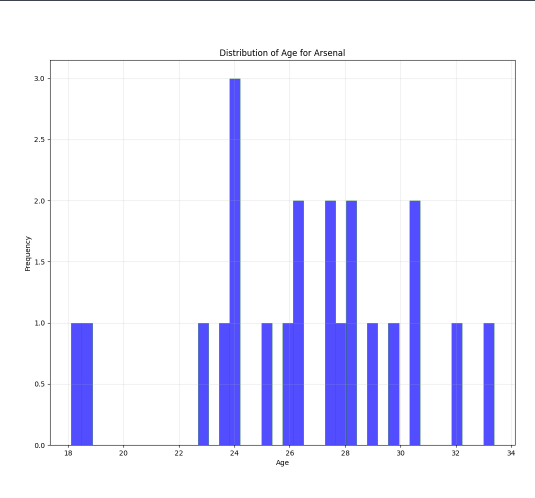
\includegraphics{ars.png}
\subsubsection{Conclusion}

The methodology for generating histograms allows for the visualization of the distribution of player statistics, both for the entire league and for each individual team. By generating these histograms, we can better understand the distribution of various performance metrics and make data-driven insights about the league and teams. The histograms are saved in organized directories for easy access and further analysis.

\subsection{Identify the highest score team}
In this section, we explain the methodology used to identify the team with the highest overall performance based on statistical analysis. This is done by comparing the mean, median, and standard deviation of performance statistics for each team and determining which team performs the best across these metrics.

\subsubsection{Overview of the Analysis}

The analysis begins by calculating the mean, median, and standard deviation for various statistics, such as goals scored per 90 minutes (GA90), red and yellow cards, and other relevant metrics, for each team. The team with the highest scores across these metrics is considered the best performing team.

The process follows a logical sequence:
1. **Calculating the Mean, Median, and Standard Deviation**: For each statistic, the mean, median, and standard deviation are calculated for each team. These values are essential for evaluating the overall performance of the team.
2. **Identifying the Team with the Highest Scores**: We then identify which team has the highest mean, median, and standard deviation for each statistic.
3. **Aggregating the Scores**: The team that performs the best in terms of the aggregated score across all statistics is determined.

\subsubsection{Loading and Preparing the Data}

The data is loaded from a CSV file, \texttt{results2.csv}, which contains statistical performance information for football teams. The columns of the dataset are renamed to provide clarity on the performance metrics for each team.

\begin{verbatim}
df = pd.read_csv('results2.csv', header = 0)
df.columns = ['Team'] + list(df.columns[1:])
team_df = df[df[df.columns[0]] != 'all']
\end{verbatim}

Non-team data rows (such as the 'all' row that aggregates stats for all teams) are removed, and the team-related statistics columns are isolated for further analysis.

\subsubsection{Identifying the Best Team for Each Statistic}

To identify the highest scoring team for each statistic, we first group the statistics into three categories: mean, median, and standard deviation.

\begin{verbatim}
columns = [col for col in df.columns if col != 'Team']
mean_cols = [col for col in columns if col.startswith('Mean of')]
median_cols = [col for col in columns if col.startswith('Median of')]
std_cols = [col for col in columns if col.startswith('Std of')]
\end{verbatim}

For each statistic, we determine the team with the highest score based on the following criteria:
- For most statistics, the highest value indicates better performance (e.g., goals scored per 90 minutes).
- For certain statistics like goals against per 90 minutes (GA90), red cards, and yellow cards, a lower value is preferred.

The code below handles the identification of the highest scoring team for each metric:

\begin{verbatim}
highest_mean = {}
highest_median = {}
highest_std = {}

def get_stats(col_name):
    return col_name.split(' of ', 1)[1]  # Get the statistic name

# Identify the team with the highest mean score
for col in mean_cols:
    stat = get_stats(col)
    if stat in ["GA90", "Age", "Red Cards", "Yellow Cards"]:
        team = team_df.loc[team_df[col].idxmin(), "Team"]
        value = team_df[col].min()
    else:
        team = team_df.loc[team_df[col].idxmax(), "Team"]
        value = team_df[col].max()
    highest_mean[stat] = (team, value)

# Identify the team with the highest median score
for col in median_cols:
    stat = get_stats(col)
    if stat == "GA90":
        team = team_df.loc[team_df[col].idxmin(), "Team"]
        value = team_df[col].min()
    else:
        team = team_df.loc[team_df[col].idxmax(), "Team"]
        value = team_df[col].max()
    highest_median[stat] = (team, value)

# Identify the team with the highest standard deviation score
for col in std_cols:
    stat = get_stats(col)
    if stat == "GA90":
        team = team_df.loc[team_df[col].idxmin(), "Team"]
        value = team_df[col].min()
    else:
        team = team_df.loc[team_df[col].idxmax(), "Team"]
        value = team_df[col].max()
    highest_std[stat] = (team, value)
\end{verbatim}

\subsubsection{Aggregating Scores Across All Statistics}

After identifying the highest performing team for each individual statistic (mean, median, and standard deviation), we aggregate the results to determine the overall best team. Each team is assigned a score based on their performance in each statistic. The team with the highest total score is considered the best.

\begin{verbatim}
top_sort = {}
for stat, (team, value) in highest_mean.items():
    if team not in top_sort:
        top_sort[team] = 0
    top_sort[team] += value

for stat, (team, value) in highest_median.items():
    if team not in top_sort:
        top_sort[team] = 0
    top_sort[team] += value

for stat, (team, value) in highest_std.items():
    if team not in top_sort:
        top_sort[team] = 0
    top_sort[team] += value

best_team = max(top_sort, key=top_sort.get)
\end{verbatim}

This aggregation is done by summing the values of the highest scores across all three categories (mean, median, and standard deviation) for each team. The team with the highest total is selected as the best team.

\subsubsection{Saving the Results}

Finally, the results of the highest performing teams in each category (mean, median, standard deviation) are saved to a text file for further analysis and reporting. Additionally, the best team overall is identified and printed.

\begin{verbatim}
# Save the result of highest mean, median and std team to a text file
with open('Best statistics.txt', 'w') as file:
    file.write('Best mean:\n')
    for stat, (team, value) in highest_mean.items():
        file.write(f'{stat}: {team} ({value})\n')
    file.write('\nBest median:\n')
    for stat, (team, value) in highest_median.items():
        file.write(f'{stat}: {team} ({value})\n')
    file.write('\nBest std:\n')
    for stat, (team, value) in highest_std.items():
        file.write(f'{stat}: {team} ({value})\n')
    file.write(f'Best team: {best_team}')
\end{verbatim}

\subsection{Conclusion}

By comparing the performance of football teams across different statistical measures (mean, median, and standard deviation), we are able to identify the team that consistently performs the best. This analysis takes into account not only the highest scores in individual statistics but also the consistency of the team's performance. The methodology allows for a comprehensive evaluation of team performance, providing insights into which team stands out in terms of overall statistical excellence.

\newpage

\section{Clustering}
\subsection{Plot 2D cluster of the data points}

In this section, we outline the methodology used to perform clustering on football player statistics using the K-means algorithm and visualize the resulting clusters in a two-dimensional space.

\subsubsection{Overview of K-means Clustering}

K-means clustering is an unsupervised machine learning algorithm that partitions the data into a predefined number of clusters. Each cluster is represented by its centroid, and data points are assigned to the cluster whose centroid is nearest. The K-means algorithm minimizes the within-cluster sum of squares (inertia) and iterates until convergence.

The goal of this analysis is to group players based on their performance metrics and categorize them into distinct clusters. These clusters can be visualized and labeled based on common features that are prominent within each group. In the context of football player data, the clusters typically represent different player roles such as goalkeepers, defenders, and offensive players.

\subsubsection{Preprocessing the Data}

Before applying the K-means clustering algorithm, several preprocessing steps are performed on the dataset:

\begin{enumerate}
    \item **Handling Non-Numeric Data**: Non-numeric columns such as player names, team names, and positions are removed from the dataset. These features are irrelevant for the clustering process, which focuses on numerical performance metrics.
    \item **Age Conversion**: The age of each player is represented as a string (e.g., "25.4 years"). We convert the age into a numerical format by extracting the age in years, ensuring it is a usable feature for clustering.
    \item **Standardization**: The data is standardized using the \texttt{StandardScaler} from scikit-learn. This step is crucial because K-means is sensitive to the scale of the features. Standardization ensures that all features have a mean of 0 and a standard deviation of 1, preventing any one feature from disproportionately affecting the clustering process.
\end{enumerate}

\subsubsection{Determining the Optimal Number of Clusters}

The next step involves determining the optimal number of clusters, which is a critical decision in K-means clustering. One common method to determine the ideal number of clusters is the **elbow method**. This method plots the inertia (sum of squared distances of samples to their closest cluster center) for different values of \( k \) (number of clusters) and identifies the point where the inertia begins to decrease at a slower rate. This point is typically considered the optimal number of clusters.

\subsubsection{Performing K-means Clustering}

Once the optimal number of clusters is identified (in this case, \( k = 3 \), corresponding to goalkeepers, defenders, and offensive players), we apply the K-means algorithm. The algorithm groups the data points into the specified number of clusters based on their performance metrics. Each data point is assigned to a cluster based on the proximity to the cluster centroid, and the process iterates to refine these assignments.

\subsubsection{Labeling the Clusters}

After clustering the data, it is essential to assign descriptive labels to the clusters to understand their meaning. In this analysis, we consider three key categories based on player roles:
- **Goalkeepers**: Players who specialize in saving shots and preventing goals.
- **Defensive Players**: Players who are focused on defending the goal, such as defenders who make tackles and interceptions.
- **Offensive Players**: Players who are primarily responsible for scoring goals and assisting in attack.

The cluster centroids are analyzed by comparing the values of key features (e.g., Save%, Tkl, Goals) within each cluster. The cluster with the highest score in features like Save% is labeled as the "Goalkeepers" cluster, the one with the highest defensive stats (e.g., Tkl, Blocks) is labeled as "Defensive Players," and the cluster with the highest offensive stats (e.g., Goals, Assists) is labeled as "Offensive Players."

\subsubsection{Visualizing the Clusters in 2D}

The next step is to visualize the clusters in two dimensions to better understand the grouping of the data points. This is achieved using Principal Component Analysis (PCA), a dimensionality reduction technique that transforms the data into a lower-dimensional space while retaining as much variance as possible.

\begin{enumerate}
    \item **PCA Transformation**: We apply PCA to the standardized data, reducing the data to two principal components. This allows us to visualize the data points on a 2D plot while preserving the structure of the original high-dimensional data.
    \item **Plotting the Clusters**: The results of the PCA are plotted on a 2D scatter plot, with each data point color-coded based on its assigned cluster label. This enables us to visually inspect how well the K-means algorithm has separated the players into distinct groups. The axes represent the first and second principal components, which capture the majority of the variance in the data.
    \item **Cluster Labels**: The scatter plot includes a legend indicating which color corresponds to each player type (Goalkeepers, Defensive Players, Offensive Players). This helps to easily identify the role of each group of players in the visualization.
\end{enumerate}

The resulting plot provides a clear visual representation of the clusters, allowing for a better understanding of how different players group together based on their performance characteristics.

\subsubsection{Interpreting the Results}

Once the 2D plot is generated, the clusters can be analyzed to draw insights about the players' performance:
- The **separation between clusters** provides insight into the distinct roles and playing styles of different types of players. Ideally, the clusters should be well-separated, indicating that the features used in the clustering process are effective in distinguishing between player types.
- The **density of the points within each cluster** can also provide information about how similar the players are within each group. Dense clusters suggest that the players within that group share similar performance statistics, while sparse clusters may indicate more variability within the group.
- The **position distribution across clusters** is another important aspect, as it allows us to verify whether the clustering aligns with the actual player positions (e.g., goalkeepers being grouped together, offensive players in another group).

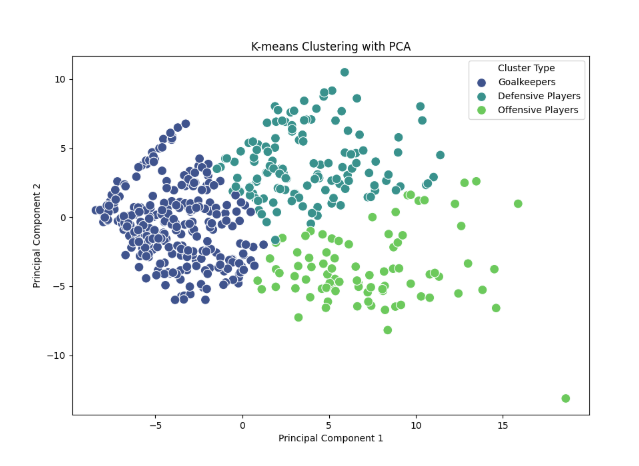
\includegraphics{k_mean.png}
\subsubsection{Conclusion}

The K-means clustering algorithm, combined with PCA for dimensionality reduction, provides an effective way to group football players based on their performance statistics. The 2D visualization of the clusters offers a clear representation of how players from different positions and playing styles are grouped. This methodology not only aids in understanding player roles but also provides a foundation for further analysis of player performance across different metrics.

The results can be used to identify patterns in player performance, highlight strengths and weaknesses within specific clusters, and inform strategies for team composition based on player characteristics.



\newpage
\section{Player Value Estimation}
\subsection{Collect player transfer values for the 2024-2025 season}


To enhance the player performance analysis with economic indicators, we collected transfer value data for football players during the 2024–2025 season. Player valuation provides an additional dimension of insight into the importance and market perception of players and allows further correlation studies between performance and economic worth.

\subsubsection{Data Source and Endpoint}

The data for player transfer values was sourced from the website \texttt{footballtransfers.com}, a popular resource for up-to-date market valuations of football players across leagues and competitions. The data was retrieved using a POST request to the following endpoint:

\begin{quote}
\texttt{https://www.footballtransfers.com/us/values/actions/most-valuable-football-players/overview}
\end{quote}

This endpoint allows fetching data in structured JSON format and includes key fields such as player names, their current clubs, and estimated transfer market values.

\subsubsection{Request Parameters and Headers}

To access the API and retrieve the relevant information, we structured our HTTP request with a custom header to mimic a browser and avoid bot detection. The payload included various filter parameters to retrieve a comprehensive dataset:

\begin{itemize}
    \item \textbf{page}: Iterated from 1 to 22 to capture paginated data.
    \item \textbf{orderBy}: Set to \texttt{estimated\_value} to sort players by their value.
    \item \textbf{tournamentId}: Set to 31, targeting the Premier League.
    \item \textbf{positionGroupId}, \textbf{mainPositionId}, \textbf{playerRoleId}, \textbf{age}, \textbf{countryId}: All set to \texttt{all} to ensure a wide and inclusive dataset.
\end{itemize}

The headers included a `User-Agent` string that mimics a standard browser and a `Referer` to signal an expected source of navigation.

\subsubsection{Data Retrieval Process}

The retrieval process was automated by iterating through multiple pages of results. For each page:

\begin{enumerate}
    \item A POST request was sent with the specified parameters.
    \item The JSON response was parsed and converted to a Pandas DataFrame.
    \item The individual page results were concatenated into a single comprehensive dataset.
\end{enumerate}

A total of 22 pages were scraped, ensuring that the top-tier and mid-tier players were included.

\subsubsection{Data Cleaning and Structuring}

After assembling the raw dataset, we focused on retaining the most relevant fields for subsequent merging with performance data:

\begin{itemize}
    \item \textbf{player\_name}: The name of the football player.
    \item \textbf{team\_name}: The team to which the player is affiliated.
    \item \textbf{estimated\_value}: The current market value of the player in euros (as estimated by the source).
\end{itemize}

All other extraneous metadata and internal IDs were removed. The cleaned DataFrame was exported as \texttt{transfer\_table.csv} for permanent storage and later access.

\subsubsection{Integration with Performance Data}

To utilize this transfer value information in conjunction with the existing player statistics (from \texttt{results.csv}), the following preprocessing and merging operations were applied:

\begin{enumerate}
    \item \textbf{Preprocessing}: Player names were standardized (e.g., trimming whitespace, correcting format) to ensure accurate matching.
    \item \textbf{Merging}: The cleaned transfer value dataset was merged with the performance dataset using a common key — typically the player name and/or team name. This step resulted in a merged DataFrame containing both performance statistics and market valuation for each player.
\end{enumerate}

This integrated dataset serves as a foundation for exploring correlations between player value and their on-field contributions, enabling more holistic assessments of player impact and cost-efficiency.

\subsubsection{Conclusion}

By systematically collecting and merging transfer value data, we are now equipped to conduct deeper analyses on how market value aligns with performance metrics. This addition enriches the analytical scope of the project, bridging the gap between athletic performance and financial valuation.

\subsection{Propose a method for estimating player value}

To understand the relationship between on-field performance and market valuation, and to propose a reliable method for estimating a football player's transfer value, we employed a supervised machine learning approach. Specifically, we used a regression model to learn the mapping between various performance metrics and a player's market value.

\subsubsection{Objective}

The goal is to predict the market value of a player using objective performance features collected from match statistics. This allows the identification of players whose market valuation may be overestimated or underestimated relative to their actual contribution on the field.

\subsubsection{Feature Selection}

Based on domain expertise and prior analysis, we selected a set of 15 performance metrics as features (independent variables) for value prediction:

\begin{itemize}
    \item \textbf{Attacking Metrics}: Goals, Expected Goals (xG), Goals per 90 minutes, Assists, Expected Assists (xAG)
    \item \textbf{Possession Metrics}: Carries, Touches, Pass Completion (Cmp), Completion Percentage (Cmp\%)
    \item \textbf{Defensive Metrics}: Tackles (Tkl), Blocks
    \item \textbf{Passing Progression}: Passes into final third (one\_third)
    \item \textbf{Goalkeeping Metrics}: Save Percentage (Save\%), Clean Sheet Percentage (CS\%), Goals Allowed per 90 minutes (GA90)
\end{itemize}

These features cover key areas of the game including offense, defense, distribution, and goal prevention, thus providing a comprehensive profile of a player's contributions.

\subsubsection{Target Variable and Data Preprocessing}

The target variable for regression was the player's \textbf{estimated market value}, extracted from the merged dataset containing both performance and economic data.

\begin{itemize}
    \item Non-numeric values (e.g., \texttt{N/a}) were replaced with zeros to ensure consistency.
    \item The dataset was split into training and testing sets with an 80-20 ratio using \texttt{train\_test\_split}.
    \item Features were standardized using \texttt{StandardScaler} to normalize value distributions and optimize model training.
\end{itemize}

\subsubsection{Model Selection and Training}

We selected the \textbf{Random Forest Regressor}, a robust ensemble learning algorithm that reduces overfitting and handles non-linear relationships well.

\begin{itemize}
    \item The model was configured with 100 decision trees (\texttt{n\_estimators=100}) and a fixed random seed for reproducibility.
    \item The training set was used to fit the model, and predictions were made on the testing set.
    \item The performance was evaluated using the \textbf{Mean Squared Error (MSE)} to quantify prediction accuracy.
\end{itemize}

\subsection{Feature Importance Analysis}

After training, we extracted feature importances from the model to identify which performance factors had the greatest influence on player valuation.

\begin{itemize}
    \item A bar plot was generated to visualize the contribution of each feature.
    \item This helps interpret model behavior and supports further discussions on fair valuation.
\end{itemize}
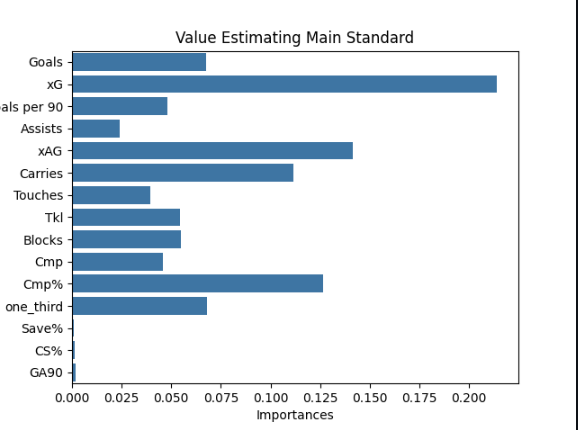
\includegraphics{image.png}

\subsubsection{Conclusion}

The proposed method demonstrates a viable approach to estimating a football player's market value based on objective performance data. By identifying the most influential features, clubs and analysts can better understand market dynamics, scout undervalued talent, and make data-driven investment decisions. The next section will explore how this model can be applied to detect anomalies in player valuation and support strategic recruitment.

\newpage
\section{Conclusion}

\subsection{Summary of Accomplishments}
This project successfully analyzed football player performance statistics to evaluate and compare team effectiveness, cluster player roles using unsupervised learning, and predict market values using regression techniques. Through systematic data preprocessing, K-means clustering, and a Random Forest Regressor model, we developed a workflow that integrates statistical performance, role categorization, and economic valuation. The model was further supported by feature importance visualization, providing insight into the key attributes driving player value.

\subsection{Learning Outcomes}
Throughout the project, we gained valuable experience in multiple areas of data science and football analytics, including:
\begin{itemize}
    \item Knowledge and techniques of scrawling data form websites.
    \item Cleaning and processing real-world sports data.
    \item Applying clustering algorithms (K-means) to uncover player role groupings.
    \item Building and evaluating a supervised learning model to predict market values.
    \item Visualizing insights using PCA and feature importance analysis.
    \item Interpreting the practical significance of statistical patterns in a sports context.
\end{itemize}

\subsection{Future Improvements}
While the project has provided strong initial results, there are several areas for future enhancement:
\begin{itemize}
    \item Incorporating more seasons and leagues to improve model generalizability.
    \item Including contextual variables such as injury history, minutes played, or club financial status.
    \item Improving value prediction accuracy by testing other models such as XGBoost or Neural Networks.
    \item Creating a dashboard interface for dynamic exploration of player and team metrics.
\end{itemize}

Overall, this work lays a solid foundation for data-driven scouting and valuation strategies in modern football analytics.

\end{document}
